\documentclass[11pt]{article}
\usepackage[margin=1in]{geometry}
\usepackage{graphicx}
\usepackage{booktabs}
\usepackage{amsmath}
\usepackage[hidelinks]{hyperref}
\usepackage{caption}
\graphicspath{{../figures/}{figures/}}
\setlength{\parskip}{4pt}

\title{Where does a reasoning model stop?\\
\large Truncation readouts of Qwen3-8B on two-option medical diagnoses --- working notes}
\author{Jingfeng Zhang}
\date{Last updated: 2026-10-08}

\begin{document}
\maketitle

\noindent These notes hold the current state of the project. Every number comes from the files named in Section~\ref{sec:files}; every figure is produced by a script in \texttt{src/} from the stored traces, so all of it can be regenerated.

\section{Setup}

\paragraph{Task.} MedXpertQA (text set, Zuo et al.\ 2025). From each 10-option question that passed a stem filter we build two-option pairs: the correct option and one of the distractors. Each pair is shown twice, once with the correct option as~A and once as~B, so position effects can be separated from content. There are 981 pairs, i.e.\ 1,962 prompts. The prompt is the question stem, the two option lines, and the instruction \emph{Answer with only A or B. No other words.}

\paragraph{Model and passes.} Qwen3-8B (revision \texttt{b968826d}) served with vLLM 0.30, run on A100 GPUs. Two passes per prompt:
\begin{itemize}
  \item \textbf{No thinking}: one greedy answer with thinking switched off (the chat template's empty \texttt{<think></think>} block). This is the model's first reaction.
  \item \textbf{Thinking}: samples with the model card's settings (temperature 0.6, top-p 0.95, top-k 20), no truncation below 32{,}768 tokens. 30 samples per prompt in the screening, 100 per prompt for the study set.
\end{itemize}

\paragraph{Readouts.} Nothing is sampled during a readout; every readout is a forward pass over stored token ids. At every sentence start of the thinking, at the stop (the position where the model wrote \texttt{</think>}) and at the answer position, we read the \emph{closed context}: prompt + thinking so far + \texttt{\textbackslash n</think>\textbackslash n\textbackslash n}, i.e.\ what the model would answer if it stopped here. From the next-token distribution we keep the raw logits $z_A, z_B$, the log probabilities, and the full-vocabulary mean, standard deviation and log-sum-exp (so the logits can be re-referenced). The \emph{gap} is $z_{\text{correct}} - z_{\text{wrong}}$, which equals the difference of log probabilities and is the log odds for the correct option. The \emph{open context} (nothing appended) gives the log probability of \texttt{</think>} itself: would the model stop here?

\paragraph{Why logits and not probabilities.} The two option probabilities are normalised against each other: at the stop $p_{\text{chosen}} \approx 1$ by construction and $p_{\text{unchosen}} \approx 1 - p_{\text{chosen}}$, so both are functions of the gap only. The question whether the \emph{chosen option's own level} is pinned at the stop (a race model) can only be asked on the logit scale. The ratio $p_{\text{chosen}}/p_{\text{unchosen}} = \exp(\text{gap})$ is the diffusion decision variable, the posterior odds for the answer.

\paragraph{Screening classes.} For every prompt we compare the greedy no-thinking answer with the 30 thinking samples (threshold 70\,\% of the samples). No-thinking wrong: \emph{helps} if $\ge 70\,\%$ of the samples answer correctly, \emph{hurts} if $\ge 70\,\%$ have a lower gap than without thinking. No-thinking right: \emph{hurts} if $\ge 70\,\%$ answer wrongly, \emph{helps} if $\ge 70\,\%$ have a higher gap. Pairs whose no-thinking answer is the same letter in both positions (199 of 981) are letter-biased and left out; their question signal is near zero (median $|{\text{gap}}|$ 0.9 against 6.5 in the other pairs).

\paragraph{Study set.} 12 pairs, one per source question, drawn with a fixed seed: group~A, 8 pairs where the no-thinking answer is wrong in both positions (gap $< -1$) and thinking is right in $\ge 70\,\%$ of the samples; group~B, 4 pairs where the no-thinking answer is right in both positions and thinking is right in $\ge 80\,\%$. Clean traces only (no truncation, median thinking 500--2{,}500 tokens), osteopathic items capped. 100 thinking samples per position give 2,400 traces with about 177{,}000 sentence positions.

\section{Findings}

\subsection{Position bias}

\begin{figure}[h]\centering
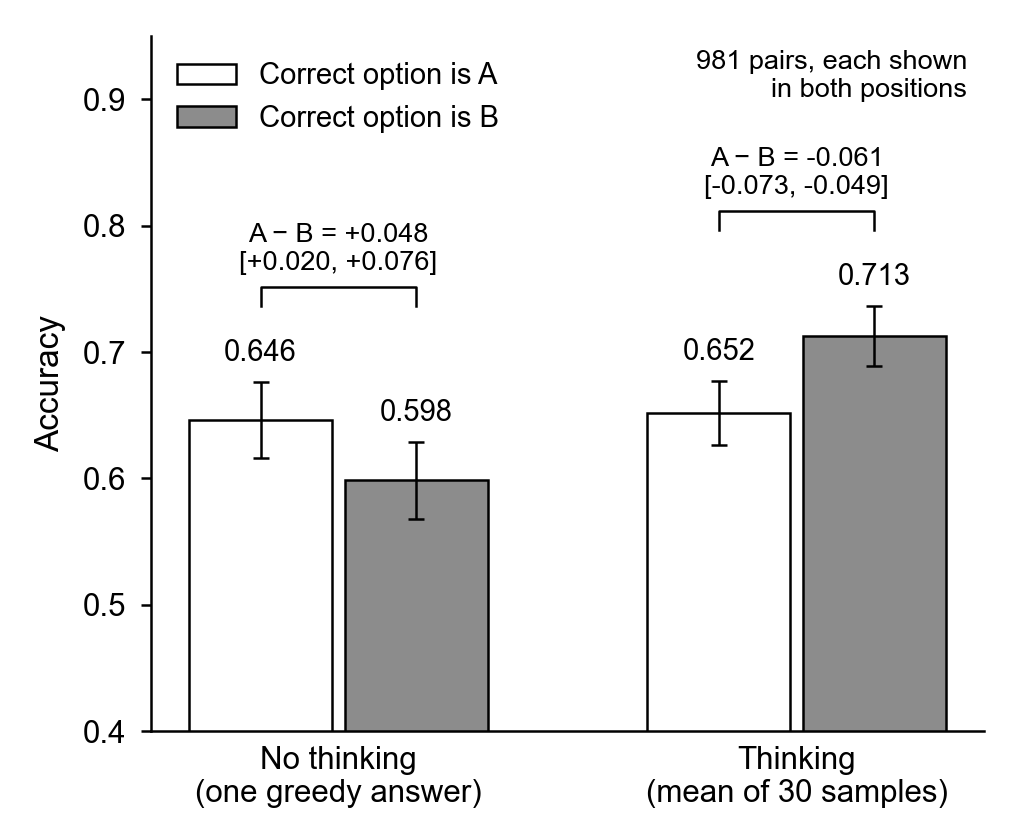
\includegraphics[width=0.5\textwidth]{fig1_position_bias.png}
\caption{Accuracy over the 981 pairs when the correct option is shown as A and as B. Error bars: 95\,\% CI over pairs; brackets: the paired difference with its CI.}
\label{fig:bias}
\end{figure}

Without thinking the model does better when the correct option is first: 0.646 against 0.598, paired difference $+0.048$ [$+0.020$, $+0.076$]. With thinking the preference reverses: 0.652 against 0.713, difference $-0.061$ [$-0.073$, $-0.049$]. The first reaction leans to A, the reasoned answer leans to B. Everything below therefore keeps both positions and requires an effect to hold in both.

\subsection{What thinking does to the evidence}

\begin{figure}[h]\centering
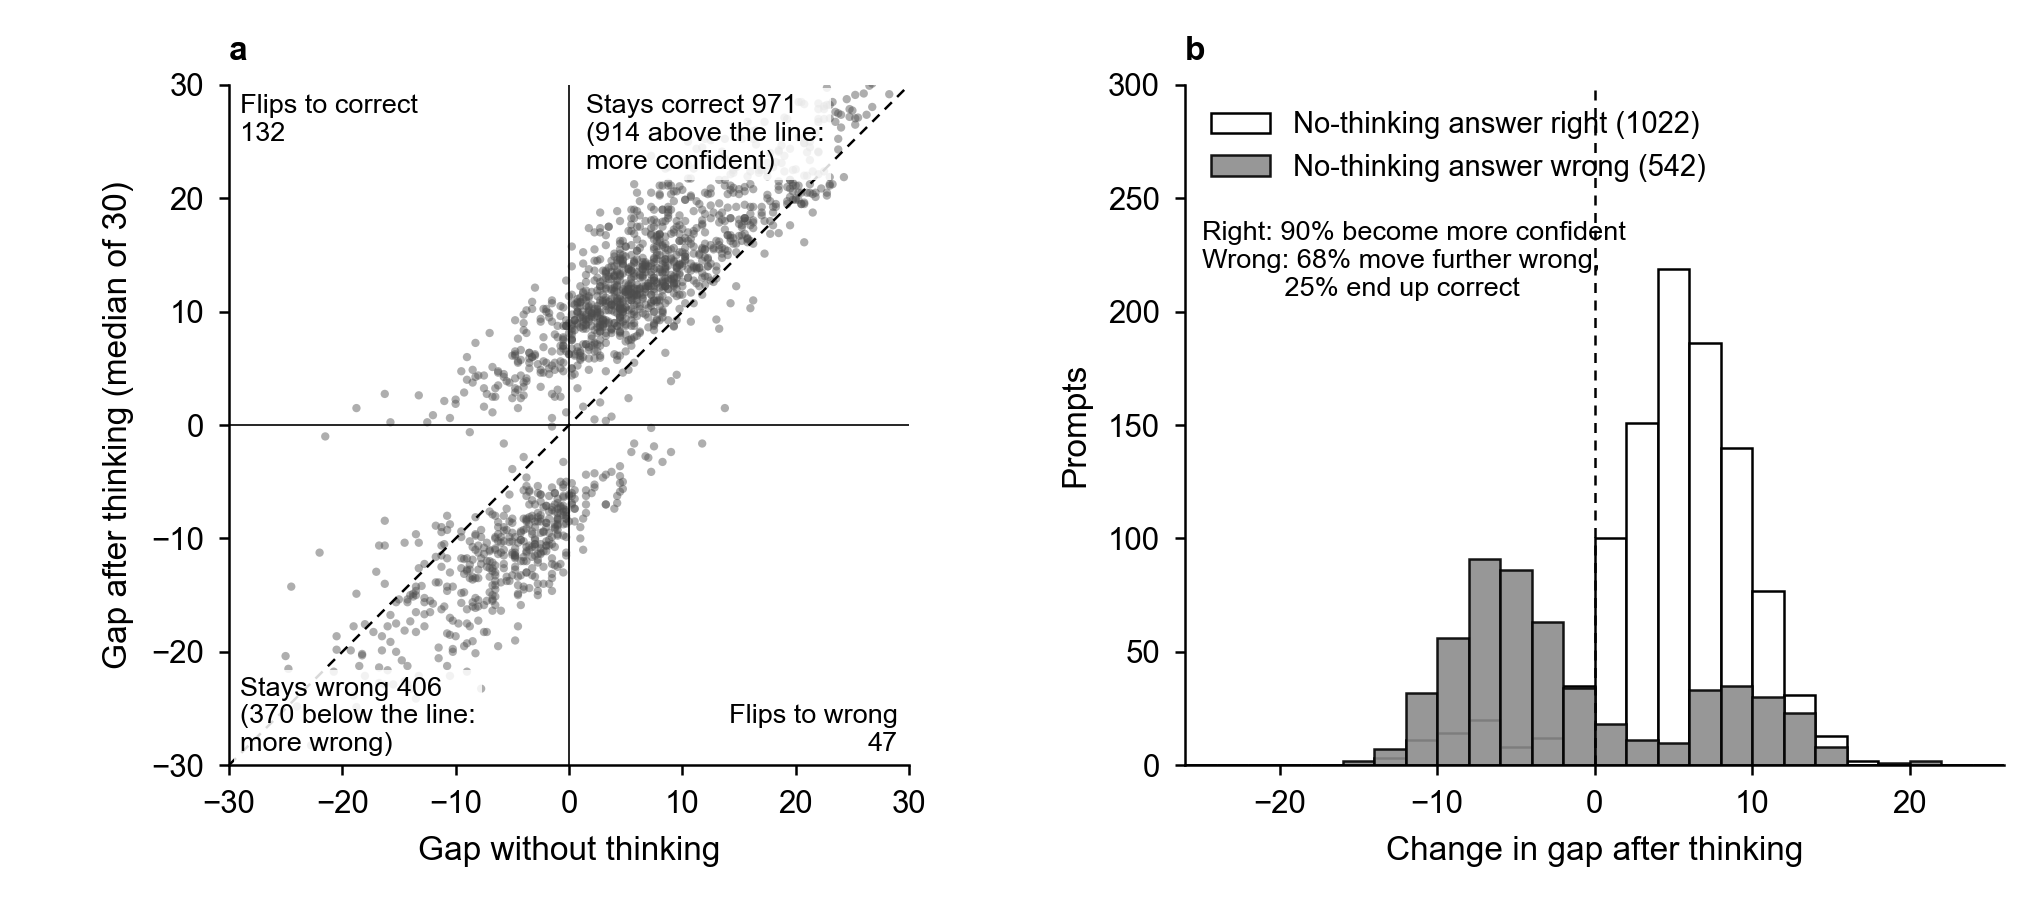
\includegraphics[width=0.95\textwidth]{fig4_gap_change.png}
\caption{Gap after thinking (median of 30 samples) against the gap without thinking, one point per prompt (a), and the change in the gap by no-thinking outcome (b). 1,564 prompts after dropping the letter-biased pairs.}
\label{fig:gapchange}
\end{figure}

Thinking roughly doubles the gap in whichever direction the first reaction pointed: median 7.4 to 13.5 when the no-thinking answer is right, $-4.8$ to $-9.9$ when it is wrong. 90\,\% of the right prompts become more confident; 68\,\% of the wrong prompts move further wrong and 25\,\% end up correct. Over the 1,564 prompts: flipped to correct 95, clearly more confident 861, no improvement 608 (256 unchanged, 352 worse). Over pairs with both positions agreeing: 420 helps (386 more confident, 34 flipped), 138 hurts (137 more wrong, 1 flipped), 172 mixed, 52 neutral.

\subsection{Accuracy of the study pairs}

\begin{figure}[h]\centering
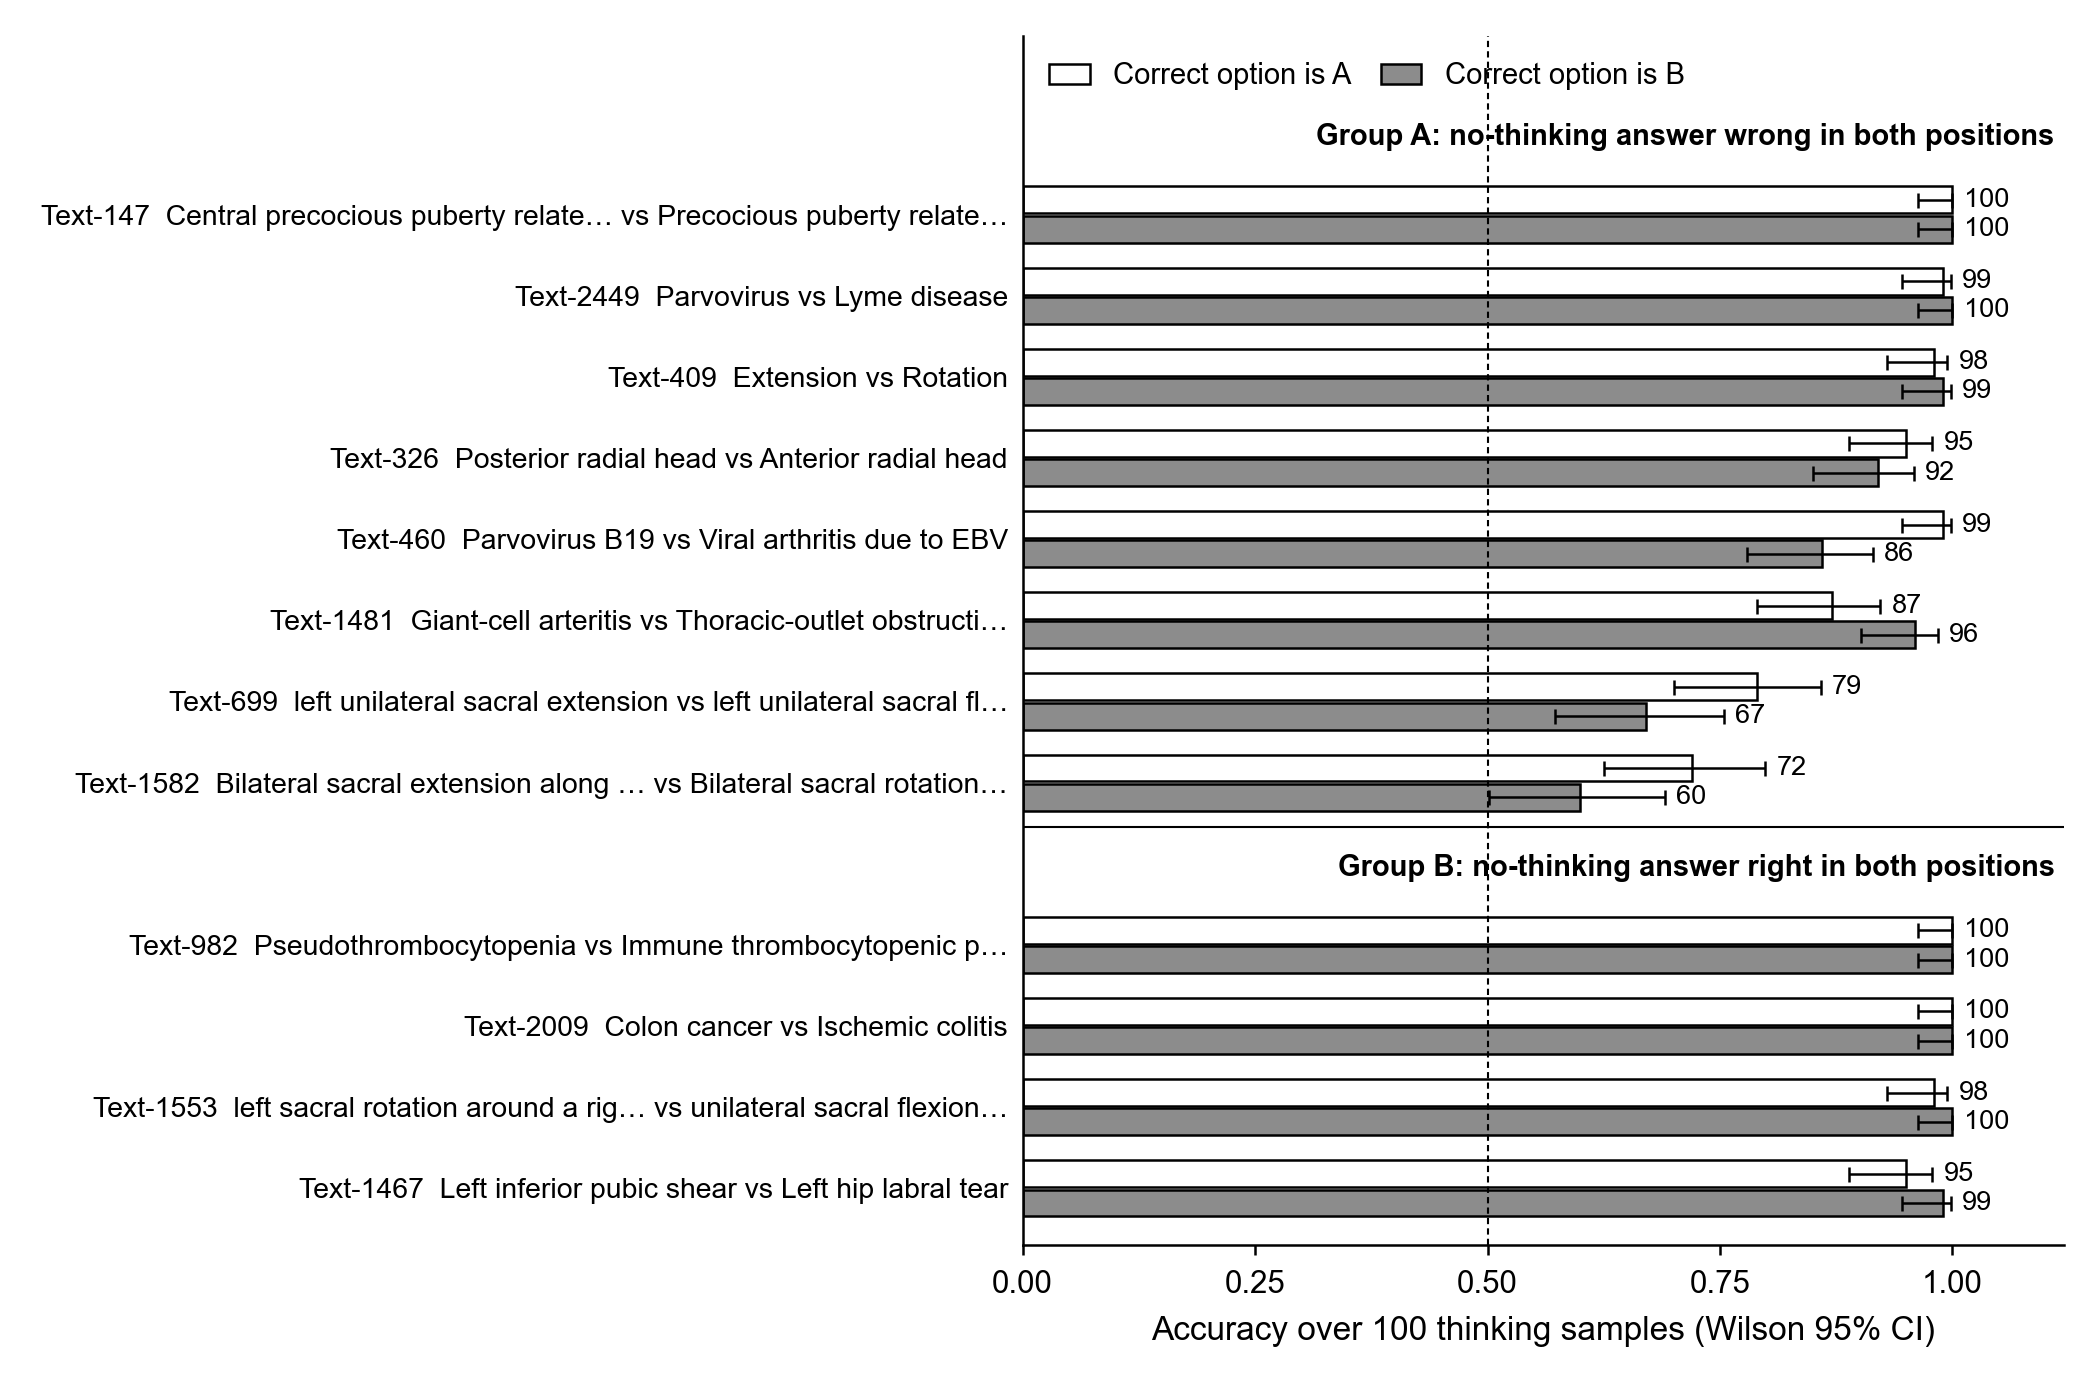
\includegraphics[width=0.8\textwidth]{fig5_study_accuracy.png}
\caption{Accuracy of the 12 study pairs over 100 thinking samples per position (Wilson 95\,\% CI).}
\label{fig:acc}
\end{figure}

Group~A: six pairs are right in 87--100\,\% of the samples, the two osteopathic pairs (Text-699, Text-1582) in 60--79\,\%. Group~B is at or near 100\,\%. Position effects survive in single pairs (Text-460: 0.99 as A, 0.86 as B; Text-1481: 0.87 and 0.96).

\subsection{Trajectories of the two option logits}

\begin{figure}[h]\centering
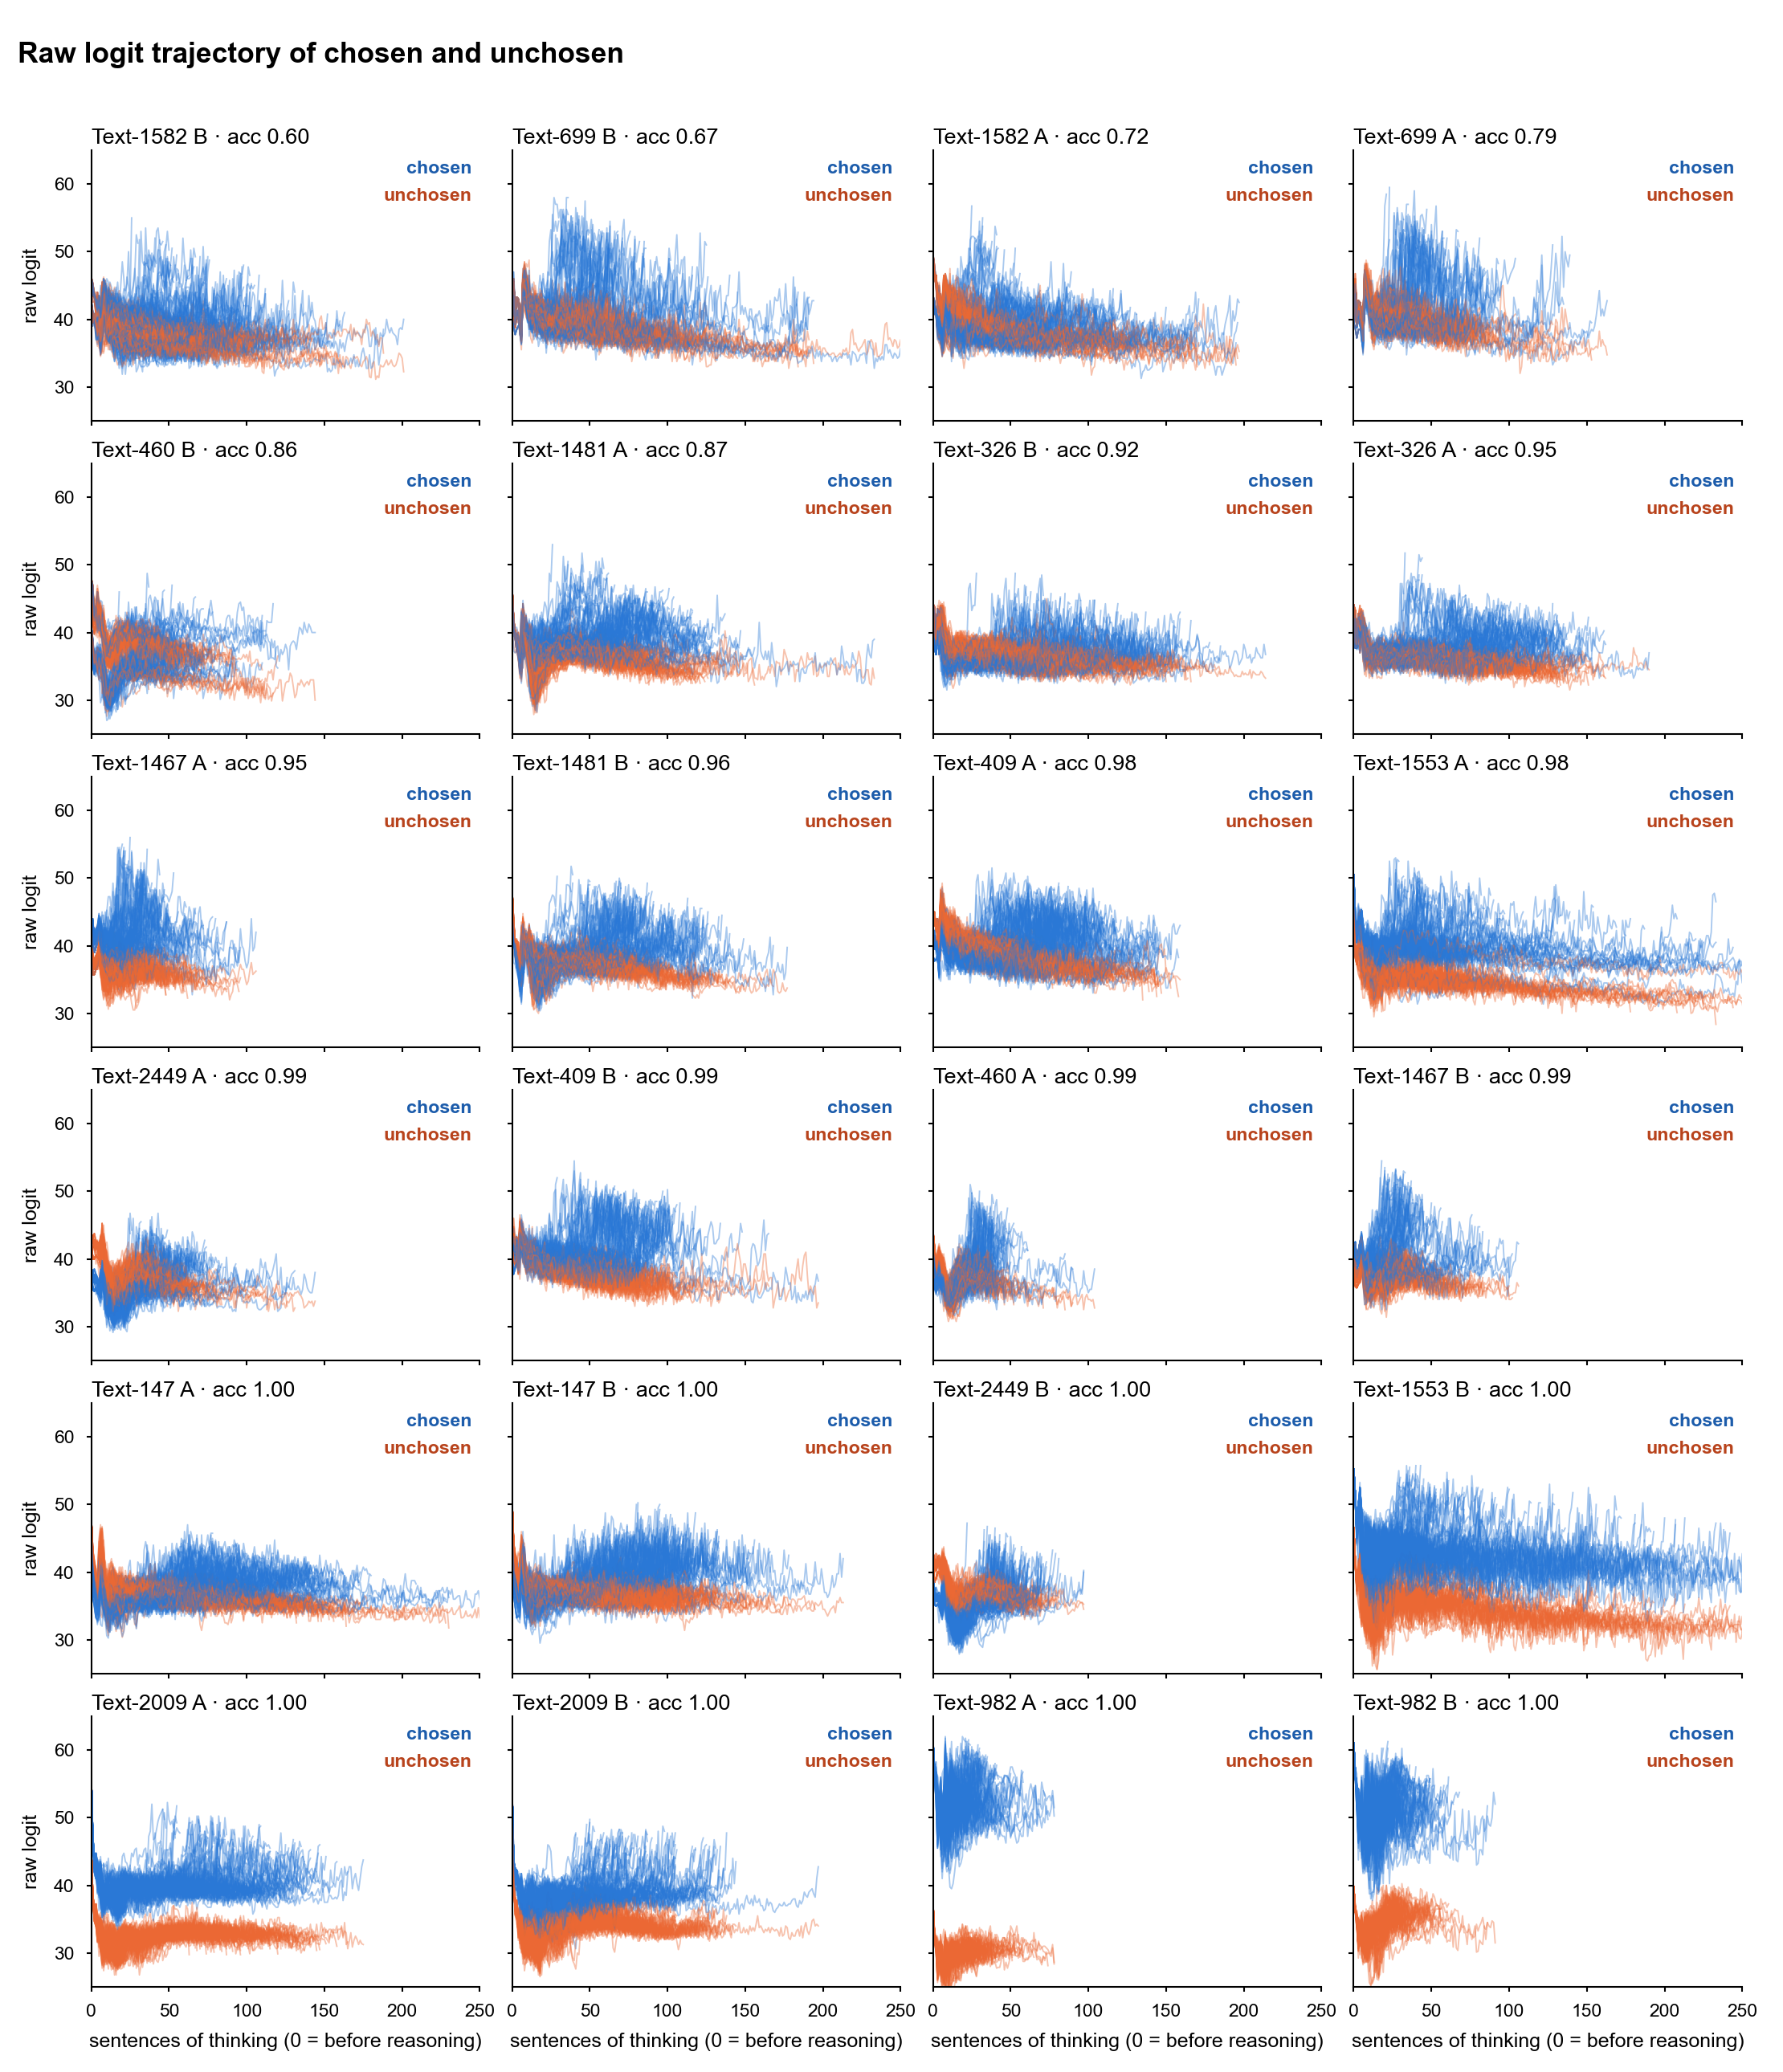
\includegraphics[width=\textwidth]{fig8_raw_logits.png}
\caption{Every sample's closed-context raw logit of the option it finally chooses (blue) and of the other option (orange), against the number of sentences of thinking kept. One panel per prompt, ordered by accuracy; all axes identical.}
\label{fig:traj}
\end{figure}

Per trace (medians over 2,400 traces): in the first half of the thinking both logits fall ($-3.5$ chosen, $-4.8$ unchosen); in the second half the chosen rises $+6.5$ while the unchosen moves $-1.0$. Sentence-to-sentence both move with similar amplitude (increment SD 1.68 and 1.39), and the increments are strongly correlated ($r = 0.82$; 59\,\% of the unchosen's increment variance is shared with the chosen). This shared movement survives referencing to the vocabulary mean, so it is specific to the two answer letters, not a drift of the whole distribution. The unchosen option sits on a floor of 34--40 in every prompt; the question-to-question differences in stop level come from how high the chosen option climbs.

\subsection{What is pinned at the stop}

\begin{figure}[p]\centering
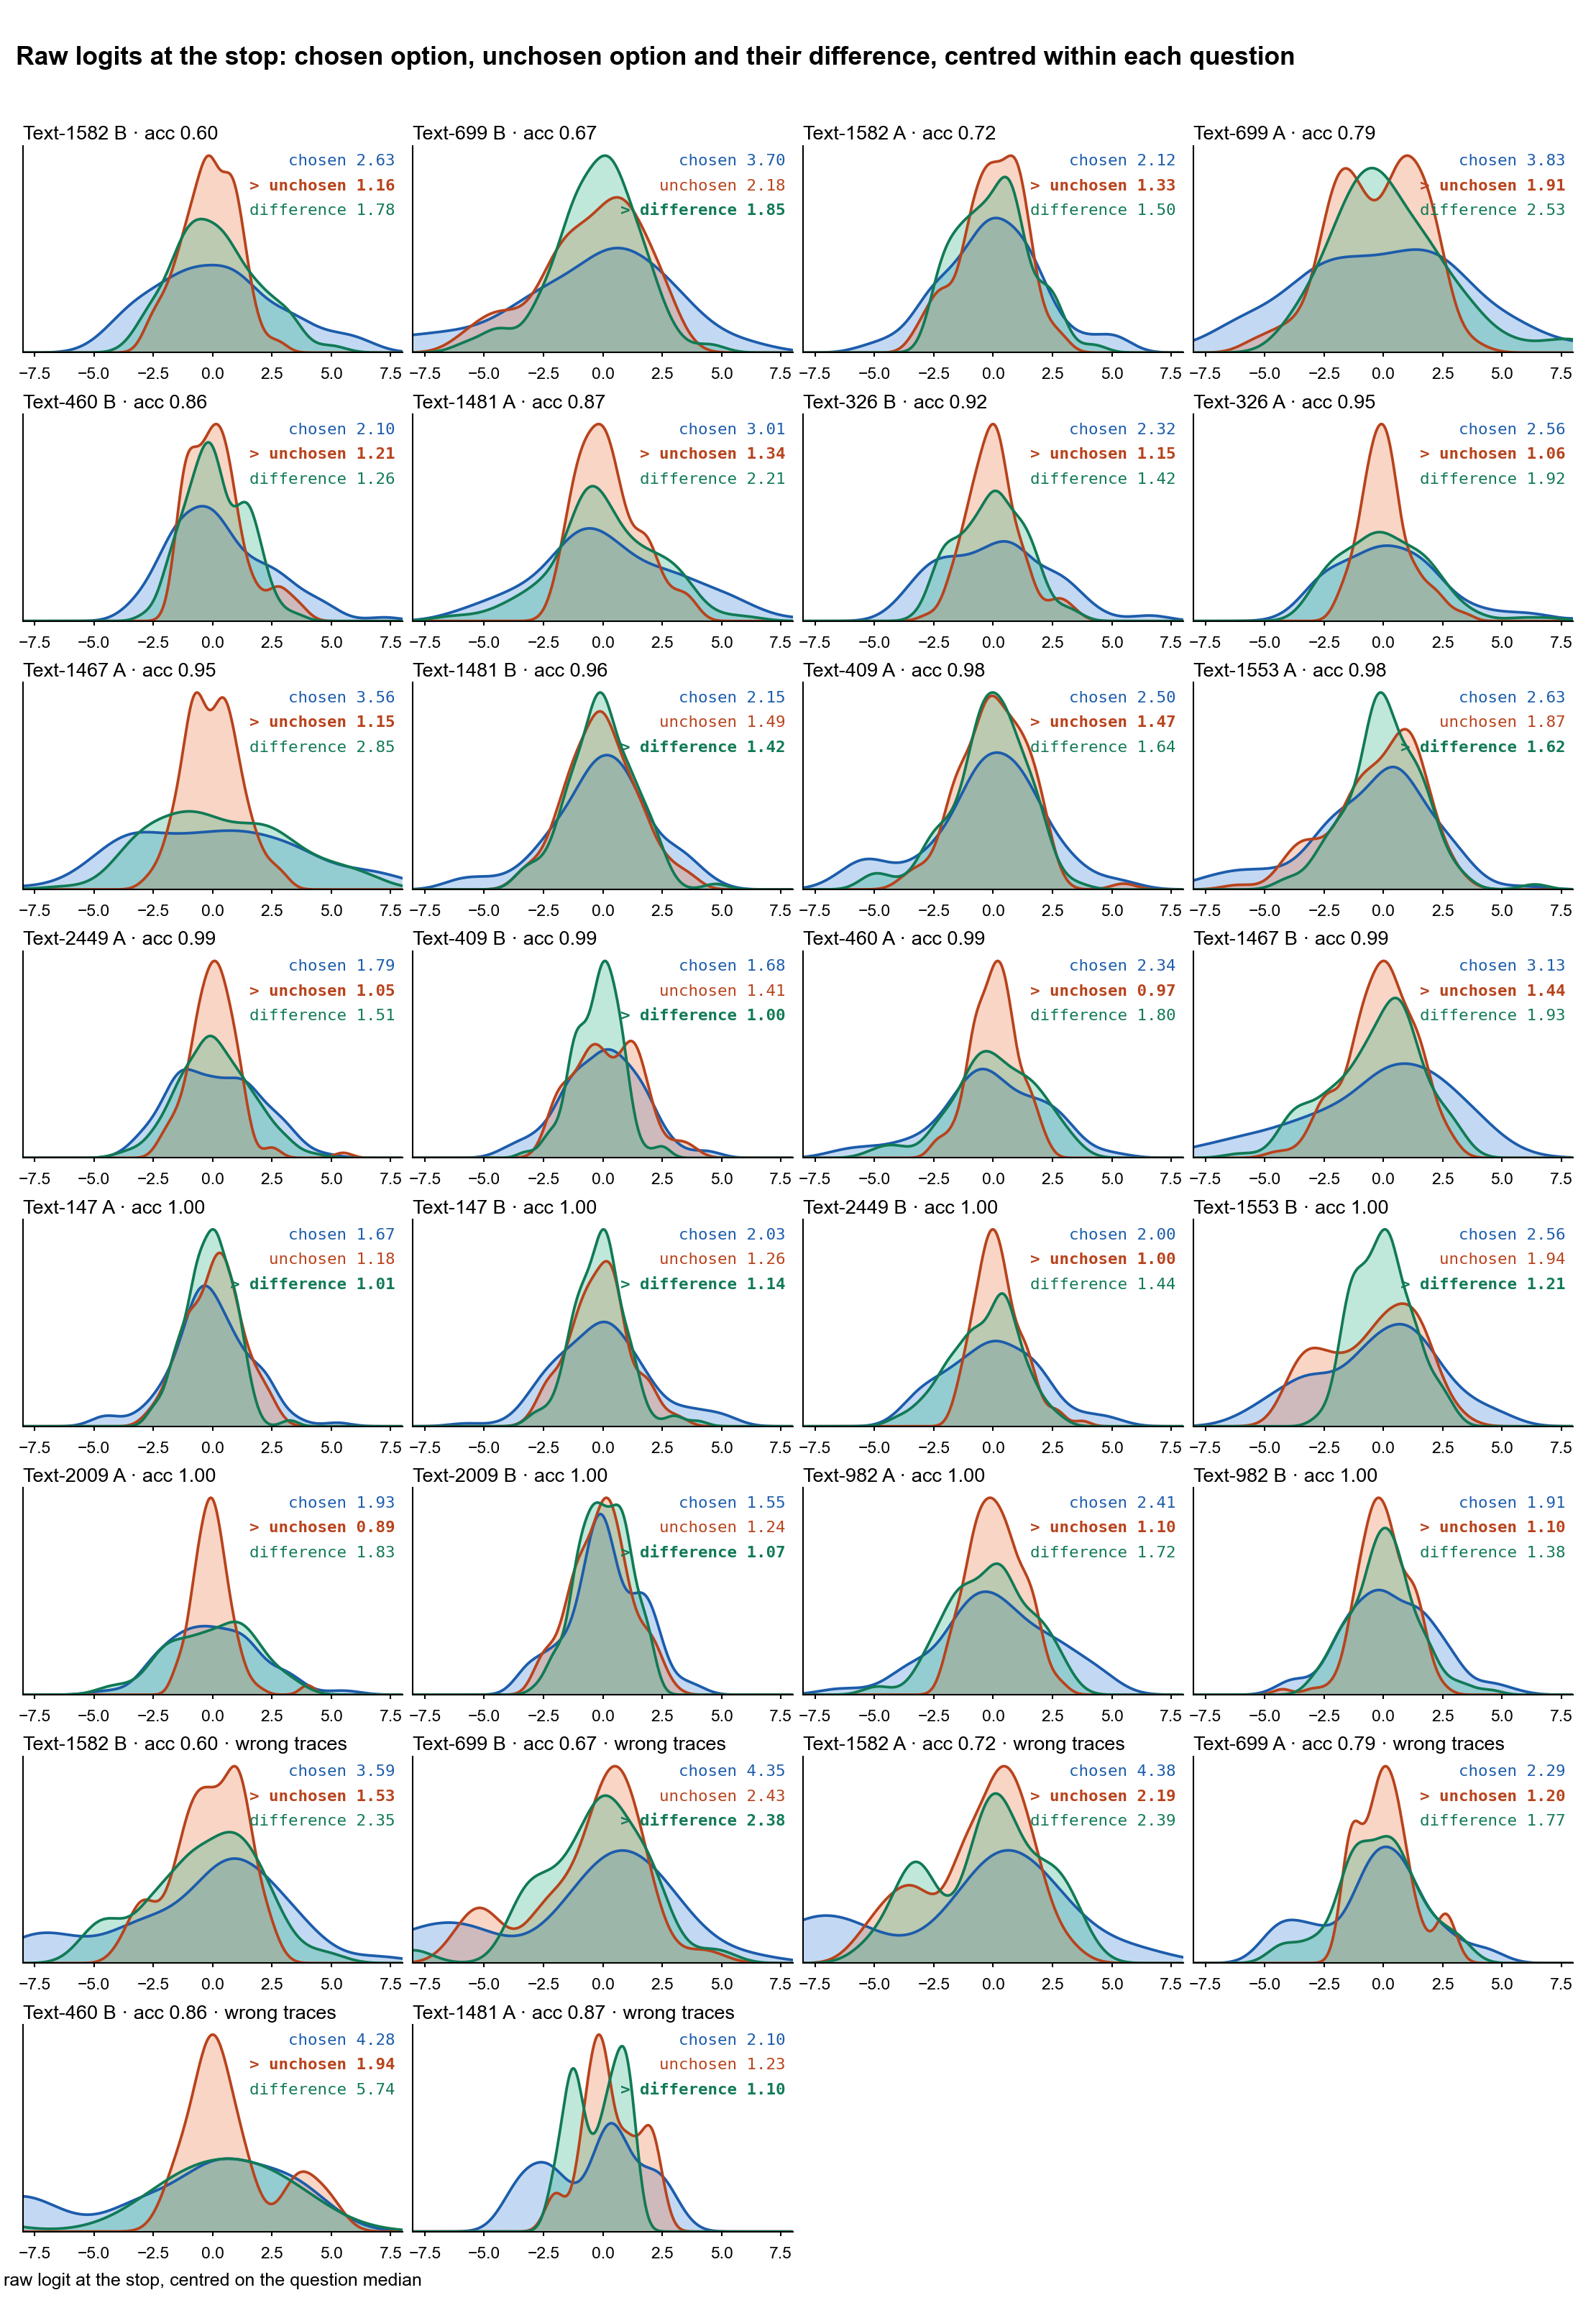
\includegraphics[width=\textwidth]{fig12_race_per_prompt.png}
\caption{At the stop, the chosen logit, the unchosen logit and their difference, each centred on its median within the prompt, one panel per prompt (traces ending right; the last rows use the traces ending wrong of the prompts with at least ten of them). The printed numbers are the three standard deviations; the tightest quantity is marked.}
\label{fig:stop}
\end{figure}

Within a prompt, the stop-point SD is 2.37 for the chosen logit, 1.68 for the difference and 1.25 for the unchosen logit (medians over 30 groups). The unchosen is the tightest quantity in 20 groups, the difference in 10, the chosen in none. The stop level also depends on when the stop happens: within prompts, later stops end lower, $r = -0.72$ for the chosen logit, $-0.69$ for the unchosen, $-0.50$ for the difference. The rise into the stop is concentrated: the last three sentences carry a median 3.2 of the 9.0 nats gained since the first sentence. Before the stop the model never considers stopping: $\log p(\texttt{</think>})$ is $-32$ at a typical sentence start (maximum $-18$ over 177{,}000 positions) and 0 at the stop.

\subsection{Errors stop at least as high as correct answers}

\begin{figure}[h]\centering
\includegraphics[width=\textwidth]{fig16_stop_diff_right_vs_wrong.png}
\caption{Stop height, $z_{\text{chosen}} - z_{\text{unchosen}}$ at the stop, for traces ending right (blue) and wrong (orange) of the same prompt; the six prompts with at least ten wrong traces. Dashed lines: medians; $p$: Mann--Whitney.}
\label{fig:rvw}
\end{figure}

\begin{table}[h]\centering\small
\begin{tabular}{lrrrrrr}
\toprule
Prompt & acc & $n$ right / wrong & gap right & gap wrong & $z_{\text{chosen}}$ right & $z_{\text{chosen}}$ wrong \\
\midrule
Text-1582 B & 0.60 & 60 / 40 & 5.0 & 12.0 & 42.6 & 48.0 \\
Text-699 B  & 0.67 & 67 / 33 & 8.8 & 12.8 & 49.2 & 52.0 \\
Text-1582 A & 0.72 & 72 / 28 & 5.5 & 10.4 & 41.8 & 50.4 \\
Text-699 A  & 0.79 & 79 / 21 & 9.5 & 11.8 & 49.0 & 52.0 \\
Text-460 B  & 0.86 & 86 / 14 & 3.0 & 11.6 & 38.8 & 43.1 \\
Text-1481 A & 0.87 & 87 / 13 & 9.5 & 7.0  & 43.8 & 42.8 \\
\bottomrule
\end{tabular}
\caption{Medians at the stop for traces ending right and wrong, same prompt. Mann--Whitney $p < 10^{-3}$ for the gap in every row; for $z_{\text{chosen}}$, $p < 0.01$ in all rows but Text-1481 A ($p = 0.06$). File: \texttt{data/screen/medxpertqa\_study12\_stop\_right\_vs\_wrong.csv}.}
\label{tab:rvw}
\end{table}

In five of the six prompts the wrong traces stop with a larger gap toward their (wrong) answer than the right traces do toward the correct one, by 2--9 nats; the chosen logit is higher too, the unchosen is the same. Errors are not premature, low-confidence stops. Pooled over all prompts the stop gap is 9.0 [6.8, 11.5] for right and 10.8 [7.5, 12.8] for wrong traces, but the pooled comparison mixes different prompts and the within-prompt table is the one to use.

\section{Model assessment}

A race model has two independent accumulators, one per option, each running toward its own bound; the first to reach its bound gives the answer and the stop. A relative-evidence (diffusion) model has one variable, the difference, running between two bounds. The table collects the predictions against what the traces show.

\begin{table}[h]\centering\small
\begin{tabular}{p{5.2cm}p{6.2cm}p{3.2cm}}
\toprule
Prediction & Observation & Verdict \\
\midrule
Race: the chosen logit is pinned at the stop, the unchosen is free & chosen SD 2.37, unchosen 1.25; chosen tightest in 0 of 30 groups & against race \\
Race: a fixed bound, so the stop level does not depend on the stop time & later stops end lower, $r = -0.72$ (chosen), $-0.50$ (difference) & against a fixed bound of either kind \\
Race: the two accumulators are independent & increments correlate $+0.82$ after removing the vocabulary mean & against race; also against a single diffusion variable, which predicts $-1$ \\
Race: the loser keeps accumulating, so longer races end with a higher loser & the unchosen has no upward drift and ends lower on later stops ($r = -0.69$) & against race \\
Both: the winner reaches the same bound whether it is the correct or the wrong option & errors stop 2--9 nats higher in 5 of 6 prompts & against both symmetric versions \\
Diffusion: the difference is pinned at the stop & difference SD 1.68, tightest in 10 of 30 groups; the unchosen is tighter & partly \\
Both: evidence accumulates gradually & the last three sentences carry 3.2 of 9.0 nats; the stop follows a verdict-like jump & against both \\
Race-like appearance: only the chosen has a net upward trend & true for the trend; but 59\,\% of the unchosen's movement is shared with the chosen & weak \\
\bottomrule
\end{tabular}
\caption{Race model and relative-evidence model against the readouts.}
\label{tab:models}
\end{table}

What fits the data best at the moment: a single relative-evidence variable in which the unchosen option has no drift of its own, a stopping threshold that falls with the length of the thinking, a common gain factor acting on both answer letters, and a stop that is triggered by a verdict sentence rather than by a level crossing. The race model's core assumption, independent accumulators finishing at a fixed bound, has no support in these traces.

\paragraph{Caveats.} (1) Raw logits have no fixed zero; referencing to the vocabulary mean leaves every number above unchanged, other references have not been tried. (2) A truncation readout is a counterfactual decision readout, not the model's internal state; the ``accumulators'' a race model posits may not be what a forced close measures. (3) Only six prompts have ten or more wrong traces. (4) Twelve pairs from one model.

\section{Next steps}
\begin{itemize}
  \item Locate the verdict sentence in every trace (the sentence carrying the final jump) and measure the distance from it to the stop in sentences and tokens.
  \item Test the collapsing-threshold reading directly: stop level as a function of stop time, within prompt, with the first-reaction level as a covariate.
  \item Repeat the stop-point analysis under a different logit reference (a neutral token's logit).
  \item Extend to the 8 group-C pairs (thinking wrong in both positions) for the error side.
\end{itemize}

\section{Files}\label{sec:files}
\begin{itemize}
  \item Generation and readouts: \texttt{src/generate.py}, \texttt{src/readout.py}; classification: \texttt{src/screen.py}; study set: \texttt{src/study\_set.py}.
  \item Figures: \texttt{src/figures.py} (fig.\ 1, 4, 5), \texttt{src/plot\_logits.py} (fig.\ 8), \texttt{src/plot\_race\_per\_prompt.py} (fig.\ 12), \texttt{src/plot\_right\_vs\_wrong.py} (fig.\ 16); all under \texttt{figures/}.
  \item Tables: \texttt{data/screen/medxpertqa\_prompts.csv}, \texttt{medxpertqa\_pairs.csv}, \texttt{medxpertqa\_study12.csv}, \texttt{medxpertqa\_study12\_stop\_height.csv}, \texttt{medxpertqa\_study12\_stop\_right\_vs\_wrong.csv}.
  \item Traces and readouts (not in git): \texttt{runs/medxpertqa/main-qwen3-8b-ab}, \texttt{-ba}.
\end{itemize}

\end{document}
